\section{Análise experimental}
\label{sec:imagelocatesubimage/experimental}

O gráfico seguinte foi gerado com a ajuda do \textit{LibreOffice Calc}. Para tal, foram primeiro gerados ficheiros, em formato csv, com os dados obtidos através da biblioteca \textit{time} da linguagem C. Depois foi gerado o gráfico a partir desse ficheiro, com resultados de 20 testes diferentes. Foi usado um computador com as seguintes especificações:

\begin{itemize}
    \item \textbf{CPU:} AMD Ryzen 7 5700U (16) @ 4.3GHz
    \item \textbf{GPU:} AMD Radeon RX Vega 8 [Lucienne]
    \item \textbf{RAM:} 16GB
\end{itemize}

\begin{figure}[H]
    \centering
    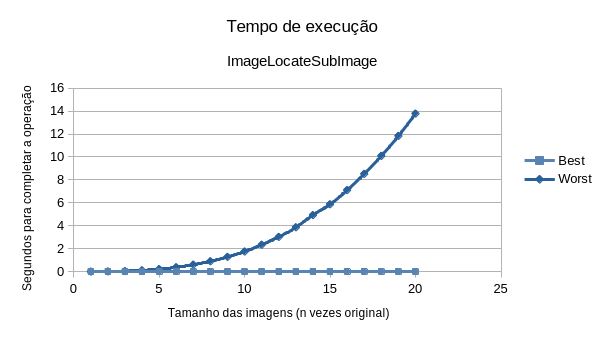
\includegraphics[width=\linewidth]{images/locatesubimage_chart.png}
    \caption{Gráfico do tempo de execução em função do tamanho das imagens fonte.}
    \label{fig:imageblur/locatesubimage_chart}
\end{figure}

Antes de fazer a análise do gráfico, é importante entender os valores. No eixo das abcissas está representado o tamanho das imagens fonte, ou seja, a imagem original, uma subimagem, e uma outra imagem que não pertence à imagem original. Para começar, a imagem original tem um tamanho de 300x300, a subimagem um tamanho de 50x50 (retirada do canto superior esquerdo da imagem original, de forma a obter o \textit{best case scenario}), e a outra imagem tem um tamanho de 100x100 (de forma a obter o \textit{worst case scenario}). Multiplica-se, então, o tamanho das imagens por cada um dos números de 2 a 20. No final, obtemos os tamanhos máximos de 6000x6000, 1000x1000 e 2000x2000, respetivamente. No eixo das ordenadas está representado o tempo de execução, em segundos, para os melhores e piores casos.

Como podemos ver na figura \ref{fig:imageblur/locatesubimage_chart}, o tempo de execução aumenta exponencialmente. Isto acontece porque o tempo de execução é proporcional ao tamanho das imagens fonte, logo se duplicarmos o tamanho de ambas as imagens, o tempo de execução passa a ser 8 vezes superior.